% =========================================================================== %
% Yes. This is a document.

\documentclass[
	english,
	aspectratio=169,
	table
]{beamer}

% =========================================================================== %
% Theme
\usepackage{scrlfile}
	\ReplacePackage{beamerthemeSHUR}{./sty/beamerthemeSHUR}
	\ReplacePackage{beamerinnerthemefancy}{./sty/beamerinnerthemefancy}
	\ReplacePackage{beamerouterthemedecolines}{./sty/beamerouterthemedecolines}
	\ReplacePackage{beamercolorthemechameleon}{./sty/beamercolorthemechameleon}

\usetheme[
	pageofpages=/,
	bullet=circle,
	titleline=true,
	alternativetitlepage=true,
	watermark="",
	watermarkheight=0px,
	watermarkheightmult=0
	]
{SHUR}

% =========================================================================== %
% the usual stuff

\usepackage[utf8]{inputenc}
\usepackage[T1]{fontenc}
\usepackage{babel}
\usepackage{lmodern}
\usepackage{microtype}
\usepackage{csquotes}
\usepackage{xspace}

\usepackage{tabularx}
\usepackage{booktabs}
\usepackage{multirow}

\usepackage{color, colortbl}
\usepackage{xcolor}
	\definecolor{tabhighlight}{RGB}{230,240,255}

\usepackage{tabto}

\usepackage{minted}
	\usemintedstyle{friendly}

\usepackage{tikz}
	\usetikzlibrary{positioning}
	\usetikzlibrary{matrix}
	\usetikzlibrary{shapes.geometric}
	\usetikzlibrary{backgrounds}
	\usetikzlibrary{calc}
	\usetikzlibrary{decorations.pathreplacing}
	\tikzstyle{every picture}+=[remember picture] 
\usepackage{adjustbox}

\usepackage{amsmath}
\usepackage{physics}

\usepackage[most]{tcolorbox}
	\tcbsetforeverylayer
		{colback=cyan!10!white,
		 colframe=cyan!75!black,
		 arc=0pt,
		 outer arc=0pt
		}
	\newtcolorbox{codebox}[1][Code]
		{colback=black!5!white,
		 colframe=blue!40!black,
		 title=#1,
		 leftupper=6mm
		}
	\newtcolorbox{cmdbox}[1][Command Line]
		{colback=black,
		 coltext=white,
		 fontupper=\ttfamily ,
		 colframe=blue!40!black,
		 title=#1,
		 outer arc=0pt
		}
	\newtcolorbox{warnbox}[1][Warning]
		{colback=black!5!white,
		 colframe=red!40!black,
		 title=#1
		}
	\newtcolorbox{hintbox}[1][Hint]
		{colback=black!5!white,
		 colframe=green!40!black,
		 title=#1
		}
	\newtcolorbox{defbox}[1][Code]
		{colback=cyan!10!white,
		 colframe=cyan!90!black,
		 title=#1
		}
%==============================================================================%
% GLOBAL MACROS

\newcommand*{\zB}{e.\,g. }
\newcommand*{\ie}{i.\,e. }

\newcommand{\Thus}{\ensuremath{\Rightarrow}\xspace}
\newcommand{\thus}{\ensuremath{\rightarrow}\xspace}

\newcommand*{\tabcrlf}{\\ \midrule}			% actually still allows for optional argument

\newcommand*{\inPy}[1]{\mintinline{python}{#1}}

\newcommand*{\todo}[1]{{\color{red}TODO: #1}}
\newcommand*{\sfrac}[2]{\ensuremath{{}^{#1}/_{#2}}}

% =========================================================================== %

\author{Stefan Hartinger}
\title{Python for Scientists}
\subtitle{Part 5: Signal Processing: Filtering, Fourier Analysis, Curve Fitting}
\institute{Department of Just Some Dude Who Likes to Talk}
\date{Spring 2023}

% =========================================================================== %

\begin{document}
% =========================================================================== %

\begin{frame}[t,plain]
\titlepage
\end{frame}

% =========================================================================== %

\begin{frame}{Efficiency}
%
\begin{center}
	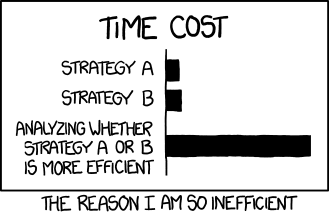
\includegraphics[width=.4\linewidth]{./gfx/02-xkcd-efficiency}\\
	\vspace{6pt}
	
	\scriptsize
	\emph{I need an extension for my research project because I spent all month trying to figure out whether learning Dvorak would help me type it faster.}

	\vspace{6pt}
	\url{https://xkcd.com/1445/}
\end{center}
%
\end{frame}

% =========================================================================== %

\begin{frame}{Scope for today}
%
\begin{itemize}
\item Analyzing efficiency
	\begin{itemize}
	\item Big $\mathcal{O}$ notation (Landau Notation)
	\item Measuring runtime in Python
	\end{itemize}
\item The weak points of Python
	\begin{itemize}
	\item The Python Object model in memory
	\item Iterators
	\end{itemize}
\item How Numpy circumvents them
	\begin{itemize}
	\item The obvious measures ...
	\item ... and the black magic
	\end{itemize}
\item Lessons to learn from this
\end{itemize}
%
\end{frame}

% =========================================================================== %

\begin{frame}[fragile]{Big $\mathcal{O}$ Notation (Landau Notation)}
%
\begin{itemize}
\item Assumption: more instructions to execute, more runtime
	\begin{itemize}
	\item This is a good assumption, but not a perfect one
	\end{itemize}
\item Repetitions multiply runtime
	\begin{itemize}
	\item \inPy{for i in range(N) : doThings()}
	\end{itemize}
\item Count only atomic instructions
	\begin{itemize}
	\item Calling a function is not atomic
	\item Count the instructions in the function instead
	\item Recursively
	\item Atomic instructions: anything you can do with a single number
		\begin{itemize}
		\item Compare
		\item add/subtract/multiply/divide
		\item copy/assign
		\end{itemize}
	\end{itemize}
\item Regard problems of \enquote{size $N$}
	\begin{itemize}
	\item E.\;g. list with $N$ elements, matrix with $K \times L$ rows/columns
	\item Get runtime as function of $N$ (or more variables, respectively)
	\end{itemize}
\end{itemize}
%
\end{frame}

% =========================================================================== %

\begin{frame}{Big $\mathcal{O}$ Notation (Landau Notation)}
%
\begin{itemize}
\item Given the exact function $T(N)$, \enquote{forget all but the dominant aspect of $T$}
	\begin{itemize}
	\item Example: $T(N) = 5 N^2 + 9.23 \cdot 10^7 N - 1 \quad \Thus \quad T \in \mathcal{O}(N^2)$
	\item Idea: \emph{Asymptotic behaviour}: for \emph{very big $N$}, lower order contributions don't matter.
	\item Prefactors less important than overall behaviour (linear, polynomial, exponential, ...).
	\item \enquote{$T$ grows at most as fast as ...}, \enquote{upper bound of rate of growth}
	\end{itemize}
\item Formal definition:
	\vspace{-4pt}
	\begin{align*}
		f(x) \in \mathcal{O}\left(\phantom{\Big.} g(x)\right)
		~
		\Leftrightarrow
		~
		\limsup_{x \to \infty} 
			\left|
				\frac
					{f(x)}
					{g(x)}
			\right|
		< \infty
	\end{align*}
	\vspace{-6pt}
\item Related:
	\begin{itemize}
	\item $\Omega(g(N)) : \limsup_{x \to \infty} \left| \dfrac{f(x)}{g(x)} \right| > 0$ \tabto{7.5cm} \enquote{lower bound of rate of growth}
	\item $o(g(N)) : \lim_{x \to \infty} \left| \dfrac{f(x)}{g(x)} \right| = 0$         \tabto{7.5cm} \enquote{negligible wrt. $g$}
	\item $\Theta(g(N)) : f \in \Theta(g) \Leftrightarrow f \in \Omega(g) ~\land~ f \in \mathcal{O}(g)$ \tabto{7.5cm} \enquote{exact rate of growth}
	\end{itemize}
	\vspace{4pt}
\item In practice, $\mathcal{O}$ and $\Theta$ are used interchangably
\end{itemize}
%
\end{frame}

% =========================================================================== %

\begin{frame}[fragile]{Big $\mathcal{O}$ Notation (Landau Notation)}
%
\vspace{-6pt}
\begin{columns}[T]
\column{.45\linewidth}
\begin{codebox}[Example: Find Minimum]
\begin{minted}[linenos, fontsize=\scriptsize]{python3}
data = [...]

def find_min(data) :
    the_min = data[0]
    idx_min = 0
    for i, x in enumerate(data) :
        if the_min > x :
            idx_min = i
            the_min = x
    return the_min, idx_min
\end{minted}
\end{codebox}
\begin{itemize}
\item Most Algorithms: Conditions
\item Implicit Assumptions:\\
	best / worst / average case
\end{itemize}
%
\column{.45\linewidth}

\begin{itemize}
\item Best case
	\begin{itemize}
	\item \texttt{data} is such that \inPy{if} condition is \inPy{False} most of the time
	\item 2 assignments before the loop
	\item 3 assigments per iteration (\texttt{i}, \texttt{x}; \inPy{enumerate})
	\item $N$ comparisons
	\item 0 assignments in the loop
	\item[\Thus] $2 + 4N$ FLOPs
	\end{itemize}
\item Worst case
	\begin{itemize}
	\item Enter \inPy{if} block every time
	\item 2 assignments per loop
	\item[\Thus] $2 + 6N$ FLOPs
	\end{itemize}
\item Either way: \texttt{find\_min }in $\mathcal{O}(N)$:\\
	linear runtime
\end{itemize}
\end{columns}
%
\end{frame}

% =========================================================================== %

\begin{frame}{Big $\mathcal{O}$ Notation (Landau Notation) - Caveats and Notes}
%
\begin{itemize}
\item Best/worst/average case assumption often not (clearly) stated, can change complexity class
\item Landau Notation only reflects \emph{asymptotic behaviour}. For small $N$, a formally worse algorithm may perform way better
\item In real life, prefactors \emph{do} matter
\item Not all operations are equal in time consumption
	\begin{itemize}
	\item Multiplications take about four times longer than addition, divisions about 10 times longer
	\item Disk I/O might be up to 100 times slower than reading from / writing to memory
	\end{itemize}
\item For overall runtime behaviour, only optimizing \emph{critical parts} (\ie code that is executed \emph{often}) is relevant
\item For runtime behaviour of recursive algorithms, see \emph{Master Theorem}
\item Same ideas apply to \emph{memory complexity classes} (how much memory is required by the algorithm)
\item Allocating memory does take (considerable!) time, too
\end{itemize}
%
\end{frame}

% =========================================================================== %

\begin{frame}{Big $\mathcal{O}$ Notation (Landau Notation) - Examples}
%
%\vspace{-6pt}
\small
\begin{columns}[T]
\column{.3\linewidth}
\begin{itemize}
\item Index access (\inPy{list})\\
 	\inPy{data[7]}\\
	$\mathcal{O}(1)$ (constant)
\item Key access (\inPy{dict})\\
 	\inPy{words["foo"]}\\
	$\mathcal{O}(1)$ (constant)
\item Searching (\inPy{list})\\
	\inPy{number in data}\\
	$\mathcal{O}(N)$ (linear)
\item Searching (\inPy{set})\\
	\inPy{number in dataSet}\\
	$\mathcal{O}(\log N)$ (logarithmic)
\end{itemize}
%
\column{.3\linewidth}
\begin{itemize}
\item Inserting (\inPy{list})\\
	\inPy{data.insert(num, pos)}\\
	$\mathcal{O}(N)$ (linear)
\item Appending to a \inPy{list}\\
	\inPy{data.append(num)}\\
	$\mathcal{O}(1)$ (constant)
\item Sorting (\inPy{list})\\
	\inPy{data.sort()}\\
	$\mathcal{O}(N \log N)$ (linearithmic)
\end{itemize}
%
\column{.3\linewidth}
\begin{itemize}
\item Inserting (\inPy{dict})\\
	\inPy{words["foo"] = "bar"}\\
	$\mathcal{O}(1)$ (constant)
\item Inserting (\inPy{set})\\
	\inPy{dataSet.union(other)}\\
	$\mathcal{O}(\log(N) \cdot K)$ (logarithmic / linear)
\end{itemize}
%
\begin{hintbox}[Overhead of \texttt{dict}s]
For each key, a \emph{hash} needs to be computed. This is in $\mathcal{O}(\texttt{len(key)})$.
\end{hintbox}
\end{columns}
%
\vspace{-18pt}
\begin{center}
\emph{All examples are average case.}
\end{center}
%
\end{frame}

% =========================================================================== %

\begin{frame}{Measuring Runtime}
%
\begin{itemize}
\item Manually: \texttt{time.perf\_counter()}
	\begin{itemize}
	\item Returns time in seconds since some (undefined) reference point as \inPy{float}
	\item Store time value before and after algorithm, compute difference -- voilà
	\item Nanosecond accuracy
	\item Variant: \texttt{time.perf\_counter\_ns()} -- returns \inPy{int}
	\item Variant: \texttt{time.process\_time()} and \texttt{time.process\_time\_ns()} -- excludes sleep time
	\item Do \emph{not} use \texttt{time.time()} -- too small resolution, affected by external factors
	\end{itemize}
\item Automatic: \texttt{timeit.timeit(command\_string)}
	\begin{itemize}
	\item Returns runtime of \texttt{command\_string} in seconds
	\item Optional argument \texttt{number=integer}: repetitions to increase accuracy
	\item Default repetitions: 1,000,000
	\item Optional argument \texttt{globals=globals()}: allow reading symbols of local scope
	\item Details: \url{https://docs.python.org/3/library/timeit.html}
	\end{itemize}
\item Resolving individual functions: \texttt{cProfile.run(command\_string)}
	\begin{itemize}
	\item Prints table: which functions called how often, total runtime and time per call, ...
	\item See \url{https://docs.python.org/3/library/profile.html}
	\end{itemize}
\end{itemize}
%
\end{frame}

% =========================================================================== %

\begin{frame}[fragile]{Measuring Runtime -- Copy and Paste Code}
%
\begin{codebox}[\texttt{time.perf\_counter}]
\begin{minted}[linenos, fontsize=\scriptsize]{python3}
import time

tic = time.perf_counter()
for repetition in range(N):
    do_things()
toc = time.perf_counter()

runtime = (toc - tic) / N
\end{minted}
\end{codebox}
%
\begin{codebox}[\texttt{timeit.timeit}]
\begin{minted}[linenos, fontsize=\scriptsize]{python3}
import timeit
import math

runtime = timeit.timeit('math.sqrt(9)', globals=globals())
\end{minted}
\end{codebox}
%
\end{frame}

% =========================================================================== %

\begin{frame}[fragile]{Measuring Runtime -- Copy and Paste Code}
%
\begin{codebox}[\texttt{cprofile.run}]
\begin{minted}[linenos, fontsize=\scriptsize]{python3}
import cProfile

cProfile.run('do_things()', sort='tottime')
\end{minted}
\end{codebox}
%
\begin{cmdbox}[Possible Output: \texttt{cprofile.run}]
\begin{minted}[fontsize=\tiny]{text}
         348221 function calls (332217 primitive calls) in 0.450 seconds

   Ordered by: internal time

    ncalls  tottime  percall  cumtime  percall filename:lineno(function)
     16005    0.119    0.000    0.119    0.000 main-profiler.py:11(decaying_oscillation_potential)
20000/4000    0.055    0.000    0.139    0.000 copy.py:128(deepcopy)
      2000    0.031    0.000    0.263    0.000 State.py:19(evolve)
      4000    0.018    0.000    0.105    0.000 copy.py:259(_reconstruct)
      8002    0.016    0.000    0.145    0.000 Misc.py:2(central_difference_quotient)
      4000    0.014    0.000    0.019    0.000 Particle.py:100(__iadd__)
     16004    0.013    0.000    0.130    0.000 Misc.py:8(inner)
      4000    0.013    0.000    0.190    0.000 Potential.py:146(get_force_at)
\end{minted}
\end{cmdbox}
%
\end{frame}

% =========================================================================== %

\begin{frame}[fragile]{The Weak Points of Python: The Object Model}
%
\begin{itemize}
\item Python: \emph{Everything is an Object}
	\begin{itemize}
	\item Object: \inPy{class} with (hidden) attributes: ref to type, ref to data, number of refs to object
	\end{itemize}
\item Upside: Allows very high flexibility. 
	\begin{itemize}
	\item E.\;g.: \inPy{list} can hold any data type, since it is a list of objects, and every object \enquote{knows} its own data type
	\end{itemize}
\item Downside: Every action takes several steps of indirection
	\begin{itemize}
	\item Example: \texttt{a + b}
	\item Find Object \texttt{a} in memory
	\item Find and follow reference to type (to read how to add something to \texttt{a})
	\item Find and follow reference to data of \texttt{a}
	\item Do the same for \texttt{b}
	\item Execute Code behind \inPy{(type(a)).__add__}
	\end{itemize}
\end{itemize}
%
\begin{hintbox}[Full Recursion]
\scriptsize
In Python, even \inPy{class}es and modules are \inPy{object}s. So \inPy{isinstance(type(object), object) == True}.
\end{hintbox}
%
\end{frame}

% =========================================================================== %

\begin{frame}{The Object Model: \inPy{list}s}
%
\begin{center}
\inPy{some_list[index] += 5}
\end{center}
%
\begin{itemize}
\item \texttt{some\_list} refers to an \inPy{object}
\item Read the type of \texttt{some\_list} to find out it's a \inPy{list}
\item Read the data pointer of \texttt{some\_list} to find it's contents
\item Exectute the \inPy{__getItem__} method of \inPy{list} (because of \texttt{some\_list[index]})
\item \texttt{index} is an \inPy{object}. Read type and data pointer, too
\item Get the stored element -- an \inPy{object}. Read type and data pointer; execute \inPy{__iadd__}
\item \inPy{5} is an object. Read type and data pointer.
\item Write the sum back to memory by calling \inPy{__setItem__}
\end{itemize}
%
\end{frame}

% =========================================================================== %

\begin{frame}[fragile]{Tangent: Unintuitive Behaviour Due to References}
%
\begin{tcbraster}[raster columns=2,
                  raster equal height,
                  nobeforeafter,
                  raster column skip=0.2cm]
%
\begin{codebox}[References.py]
\begin{minted}[linenos,fontsize=\scriptsize]{python3}
table_1 = [[1, 0]] * 2
table_2 = [[1, 0] for i in range(2)]

print(table_1)
print(table_2)
print()

table_1[0][1] = -1
table_2[0][1] = -1

print(table_1)
print(table_2)
\end{minted}
\end{codebox}
%
\begin{cmdbox}[Output: References.py]
\begin{minted}[fontsize=\scriptsize]{text}
[[1, 0], [1, 0]]
[[1, 0], [1, 0]]

[[1, -1], [1, -1]]
[[1, -1], [1, 0]]
\end{minted}
\end{cmdbox}
%
\end{tcbraster}
%
\end{frame}

% =========================================================================== %

\begin{frame}{Tangent: Explanation}
%
\begin{itemize}
\item \inPy{table_1 = [[1, 0]] * 2}
	\begin{itemize}
	\item Construct the element \inPy{[[1, 0]]} somewhere in memory \Thus location $A$
	\item Compute \texttt{[$A$]} \inPy{* 2} \enquote{=} \texttt{[$A$, $A$]}
	\item Store result of this computation in \texttt{table\_1}
	\item[\Thus] \texttt{table\_1} contains \emph{two references to the same object}! 
	\end{itemize}
\item \inPy{[[1, 0] for i in range(2)]}
	\begin{itemize}
	\item For each \texttt{i}, construct a new object \texttt{[1, 0]} \Thus locations $A, B$
	\item Put them together in a \inPy{list} \enquote{=} \texttt{[$A$, $B$]}
	\item[\Thus] \texttt{table\_2} contains \emph{references to two different objects}! 
	\end{itemize}
\end{itemize}
%
\begin{hintbox}[It's not a bug{,} it's a feature!]
This kind of behaviour avoids copying long lists and replaces the tedious step by copying a single number (the reference). Once you get used to it, you'll like it.
\end{hintbox}
%
\end{frame}

% =========================================================================== %

\begin{frame}[fragile]{The Weak Points of Python: Iterators}
%
\begin{itemize}
\item Remember: Iterator -- \enquote{Book keeping device}, stores how to find next object in loop
	\begin{itemize}
	\item Details: see Part 3 of this series
	\end{itemize}
\item Iterators are objects ...
\item ... with their own methods ...
\item ... and own attributes, which are again objects
\item[\Thus] A simple \inPy{for} loop does several \enquote{invisible} operations before we even touch our code! For every iteration!
\end{itemize}
%
\begin{hintbox}[Where this helps]
Iterators provide a uniform interface for traversing arbitrary structures, such as \inPy{dict}s (Hashmaps), \inPy{set}s (Red-Black-Trees), \inPy{list}s (Arrays) and even self-defined structures.
\end{hintbox}
%
\end{frame}

% =========================================================================== %

\begin{frame}[fragile]{How Numpy Circumvents Python's Weak Points}
%
\begin{itemize}
\item Numpy is written in C
	\begin{itemize}
	\item Less flexible, less overhead
	\item Numpy-Arrays are of one single type
	\item Iteration using integer indices rather than complex iterators
	\end{itemize}
\item Numpy runs directly on the processor, not in the Python RTE
	\begin{itemize}
	\item RTE: runtime environment
	\item Python is compiled to bytecode; essentially code for \enquote{Python OS}
	\item Python interpreter translates between bytecode (pseudo machine language) and local machine
	\item Numpy bypasses this, \enquote{speaks directly to the processor} 
	\end{itemize}
\item Numpy uses black magic
	\begin{itemize}
	\item SIMD and other hardware level optimizations
	\item Bonus slides at the end if you're interested
	\end{itemize}
\item[\Thus] Proper use of numpy should give you about $10\times$ speedup.
\end{itemize}
%
\end{frame}

% =========================================================================== %

\begin{frame}{Lessons to Learn: Pure Python Level}
%
\begin{itemize}
\item Avoid repeated evaluation of the same expression
	\begin{itemize}
	\item Compute constants before loops
	\item Create lookup tables for often-needed expressions
	\end{itemize}
\item Use apt data containers
	\begin{itemize}
	\item Frequent indexed read, rare inserts \Thus \inPy{list}s
	\item Frequent indexed read, frequent inserts \Thus \inPy{dict}s
	\item Frequent check: object in container? \Thus \inPy{set}s
	\item Small datasets \Thus \inPy{list}s
	\end{itemize}
\item Use builtin functions/methods
	\begin{itemize}
	\item for \inPy{list}s: \texttt{count}, \texttt{reverse}, \texttt{sort}
	\item for \inPy{dict}s: same methods via \texttt{keys}, \texttt{values}, \texttt{items}; \texttt{fromkeys(keys, values)}
	\item for \inPy{set}s: \texttt{difference}, \texttt{intersection}
	\item for all iterables: \inPy{sum}, \inPy{min}, \inPy{max}, \inPy{reversed}
	\end{itemize}
\end{itemize}
%
\end{frame}

% =========================================================================== %

\begin{frame}{Lessons to Learn: Numpy Guidelines}
%
\begin{itemize}
\item Pre-allocate rather than append/insert:\\
	Prefer \inPy{data = np.zeros(size)} or \inPy{data = np.ones(size) * initial_value} plus update over inserting 
\item Avoid frequent conversions -- start with one (numpy-) datatype and stick to it
\item Avoid copies -- use views
	\begin{itemize}
	\item \inPy{data = np.random.random(size)}
	\item \inPy{view = data[3:9:2]}
	\item No copy -- \texttt{view} describes a sub-array of \texttt{data}
	\item Changes to \texttt{view} affect \texttt{data}
	\end{itemize}
\item Use numpy-builtins rather than Python builtins or own implementations
	\begin{itemize}
	\item \texttt{sum}, \texttt{product}, \texttt{min}, \texttt{max}, \texttt{argmin}, \texttt{argmax}
	\item \texttt{sin}, \texttt{cos}, \texttt{tan}, \texttt{exp}, \texttt{exp2}, \texttt{log}, ...
	\item \texttt{dot}, \texttt{@} (aka \inPy{__matmul__}), \texttt{inner}, \texttt{outer}
	\item \texttt{around}, \texttt{angle}, \texttt{take}, ...
	\end{itemize}
\end{itemize}
%
\end{frame}

% =========================================================================== %
%
\begin{frame}[fragile]{Numpy -- Copy and Paste Patterns}
%
\begin{codebox}[Pre-Evaluate Functions]
\begin{minted}[linenos, fontsize=\scriptsize]{python3}
import numpy as np

one_dimensional = np.arange(start, stop, stride)
data = np.sin(one_dimensional)

X, Y, Z, ... = np.meshgrid(values_x, values_y, values_z, ...)
data = np.sin(X*X + Y*Y) * Z
\end{minted}
\end{codebox}
%
\begin{hintbox}[Non-Numpy Functions]
\small
This usually also works with non-numpy functions \texttt{f}.
If the Python-function \texttt{f} contains statements like \inPy{if}, you can pre-compile it with \texttt{np.vectorize}.

\vspace{6pt}
See:\\
\url{https://numpy.org/doc/stable/reference/generated/numpy.vectorize.html}
\end{hintbox}
%
\end{frame}

% =========================================================================== %


\begin{frame}[fragile]{Numpy -- Copy and Paste Patterns}
%
\begin{codebox}[Conditional Operations]
\begin{minted}[linenos, fontsize=\scriptsize]{python3}
import numpy as np

data = np.random.random((5, 5)) - 0.5
mask = data > 0
sum_of_positive_values = data[mask].sum()
\end{minted}
\end{codebox}
%
\begin{codebox}[Reductions and Partial Reductions]
\begin{minted}[linenos, firstnumber=last, fontsize=\scriptsize]{python3}
total = data.sum()
sum_of_rows    = data.sum(axis=0)    # sum_i data[i, :]
sum_of_columns = data.sum(axis=1)    # sum_i data[:, i]
\end{minted}
\end{codebox}
%
\end{frame}

% =========================================================================== %

\begin{frame}[fragile]{Numpy -- Copy and Paste Patterns}
%
\begin{codebox}[Map to nearest known value]
\begin{minted}[linenos, fontsize=\scriptsize]{python3}
import numpy as np

angles = np.arange(0, 360, 0.25)
lookup_sines = np.sin(angles)

intermediate_result = get_angle()
closest_angle_idx = np.abs(angles - intermediate_result).argmin()

print(f"sin({intermediate_result:6.2f}) ~= {lookup_sines[closest_angle_idx]:4.2f}")
\end{minted}
\end{codebox}
%
\end{frame}

% =========================================================================== %

\begin{frame}[fragile]{Example Runtime Measurements}
%
\begin{columns}[T]
\column{.43\linewidth}
\begin{codebox}[Computing Sums]
\begin{minted}[linenos, fontsize=\scriptsize]{python3}
def sum_naive(data_sum):
    result = 0
    for num in data_sum:
        result += num
    return result

def sum_builtin(data_sum):
    return sum(i for i in data_sum)

def sum_numpy(data_sum):
    return np.array(data_sum).sum()

def sum_numpy_no_allocate(
        data_sum_numpy):
    return data_sum_numpy.sum()
\end{minted}
\end{codebox}
%
\column{.5\linewidth}
\begin{center}
\small
\newcolumntype{O}{>{\centering \arraybackslash}m{.34\linewidth}}
\newcolumntype{E}{>{\raggedleft\arraybackslash}m{.24\textwidth}}
\rowcolors{1}{tabhighlight}{white}
\begin{tabularx}
	{\linewidth}
	{OEE}
	\toprule[1.5pt]
	\textbf{Approach}        & {\textbf{Time}~~~~} & \textbf{Relative} \tabcrlf
	
    \texttt{sum\_naive}      &    23.703 ms & 100.00\% \\
    \texttt{sum\_builtin}    &    21.128 ms &  89.14\% \\
    \texttt{sum\_numpy}      &    24.975 ms & 105.37\% \\
    \texttt{no\_allocate}    &     0.449 ms &   1.89\% \\
    \texttt{sum\_expression} &     0.001 ms & $^{1}/_{20000}\times$ \\
	
	\bottomrule[1.5pt]
\end{tabularx}

\vspace{6pt}
\emph{\small For $N = 1\,000\,000$}
\end{center}
%
\begin{codebox}[Computing Sums]
\begin{minted}[linenos, firstnumber=last, fontsize=\scriptsize]{python3}
def sum_expression(N):
    return N * (N - 1) // 2
\end{minted}
\end{codebox}
\end{columns}
%
\end{frame}

% =========================================================================== %

\begin{frame}[fragile]{Example Runtime Measurements}
%
\vspace{-6pt}
\begin{tcbraster}[raster columns=2,
                  raster equal height,
                  nobeforeafter,
                  raster column skip=0.2cm]
%
\begin{codebox}[Building Lists]
\begin{minted}[linenos, fontsize=\scriptsize]{python3}
def list_append(N_list):
    result = []
    for i in range(N_list) :
        result.append(i)
    return result

def list_comprehension(N_list):
    return [i for i in range(N_list)]
\end{minted}
\end{codebox}
%
\begin{codebox}[Building Lists]
\begin{minted}[linenos, firstnumber=last, fontsize=\scriptsize]{python3}
def list_numpy_arange(N_list):
    return np.arange(N_list)

def list_numpy_append(N_list):
    result = np.array([])
    for i in range(N_list):
        result = np.append(result, i)
    return result
\end{minted}
\end{codebox}
%
\end{tcbraster}
%
\begin{center}
\small
\newcolumntype{O}{>{\centering \arraybackslash}m{.41\linewidth}}
\newcolumntype{E}{>{\raggedleft\arraybackslash}m{.25\textwidth}}
\rowcolors{1}{tabhighlight}{white}
\begin{tabularx}
	{\linewidth}
	{OEE}
	\toprule[1.5pt]
	\textbf{Approach}            & {\textbf{Time}~~~~} & \textbf{Relative} \tabcrlf
	
    \texttt{list\_append}        &     3.277 ms & 100.00\% \\
    \texttt{list\_comprehension} &     2.214 ms &  67.56\% \\
    \texttt{list\_numpy\_arange} &     0.040 ms &   1.22\% \\
    \texttt{list\_numpy\_append} &  1431.615 ms & $436.87\times$ \\
	
	\bottomrule[1.5pt]
\end{tabularx}
\emph{\small For N = 10,000}
\end{center}
%
\end{frame}

% =========================================================================== %

\begin{frame}{The \emph{Real} Lesson to Learn}
%
\begin{columns}
\column{.6\linewidth}
\begin{itemize}
\item Write correctly working code first
\item Profile it
\item Only then, begin to optimize
\end{itemize}

\vspace{6pt}
\begin{hintbox}[Donald Knuth says]
\emph{We should forget about small efficiencies, say 97\% of the time: premature micro optimizations are the root of all evil.}
\end{hintbox}
%
\column{.3\linewidth}
\begin{center}
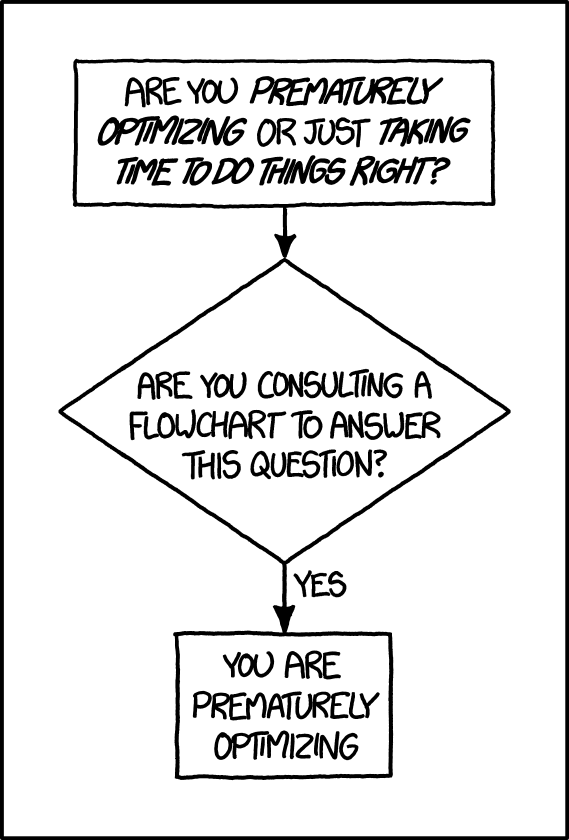
\includegraphics[width=.8\linewidth]{./gfx/02-xkcd-premature-optimization}
\scriptsize
\url{https://xkcd.com/1691/}
\end{center}
\end{columns}
%
\end{frame}

% =========================================================================== %

\begin{frame}
%
\begin{center}
\Huge
Bonus Slides
\end{center}
%
\end{frame}

% =========================================================================== %

\begin{frame}{Computer Architecture}
%
\begin{itemize}
\item Processor: \emph{very limited} capabilites
	\begin{itemize}
	\item Registers: extremely fast memory cells; usually 8 byte (64 bit)
	\item Elementary operations act on these registers
	\item Elementary operations: add, multiply, store in \enquote{regular memory}, ...
	\item Some registers for specialized use only (flags register, instruction pointer, data index, ...)
	\item Not even floating point operations!
	\end{itemize}
\item FPU (floating point unit)
	\begin{itemize}
	\item Extra chip
	\item Usually available since 32bit era
	\item Embedded devices still might not have them
	\end{itemize}
\item Caches
	\begin{itemize}
	\item Fast but small memory devices (some kB to MB)
	\item Used for often needed data
	\item[\Thus] Potential for optimization: keep data close together
	\end{itemize}
\end{itemize}
%
\end{frame}

% =========================================================================== %

\begin{frame}{SIMD -- Single Instruction Multiple Data}
%
\begin{itemize}
\item Do the same instruction (\zB addition) with \emph{multiple numbers} in parallel
\item Requires specialized hardware ...
	\begin{itemize}
	\item 1997: Intel Pentium with MMX (MultiMedia eXtensions)
	\item 1999: SSE (Streaming SIMD Extensions); Also SSE2, SSE3, SSE4
	\item 2008: AVX (Advanced Vector Extensions)
	\item All of them: specialized registers with up to 512 bits (64 byte)
	\item Set of instructions such as vector addition\\
		See \url{https://www.intel.com/content/www/us/en/docs/intrinsics-guide/index.html}
	\end{itemize}
\item ... and software
	\begin{itemize}
	\item Few codes trivially parallelizable
	\item Example array summation
		\begin{itemize}
		\item Partition array into N sublists
		\item Compute N sub-sums in parallel
		\item Sum up N numbers without parallelization
		\end{itemize}
	\end{itemize}
\end{itemize}
%
\end{frame}

% =========================================================================== %

\begin{frame}{Test Case: Sum Up Integers}
%
\begin{columns}[T]
\column{.42\linewidth}
\begin{itemize}
\item Compute $\sum_i^N i$
\item Python, Numpy, C and C with SIMD
\item Naive approach (Python and C)
	\begin{itemize}
	\item Initialize variable \texttt{result} to \texttt{0}
	\item For each \texttt{i} between \texttt{0} and \texttt{N}
		\begin{itemize}
		\item increase \texttt{result} by \texttt{i}
		\end{itemize} 
	\end{itemize}
\item Numpy approach
	\begin{itemize}
	\item \texttt{np.arange(N).sum()}
	\end{itemize}
\end{itemize}
%
\column{.48\linewidth}
\begin{itemize}
\item SIMD approach 1
	\begin{itemize}
	\item Initialize variable \texttt{result} to \texttt{0}
	\item Prepare AVX register \texttt{accumulator}: $8\times$ \texttt{0}
	\item Prepare AVX register \texttt{summand}
	\item For each \texttt{i} between \texttt{0} and \texttt{N} (stride \texttt{8})
		\begin{itemize}
		\item Set \texttt{summand[j] = i + j} for each j between \texttt{0} and \texttt{7}
		\item Add \texttt{summand} to \texttt{accumulator} parallelly
		\end{itemize}
	\item sum up \texttt{accumulator[j]} for each \texttt{j} between \texttt{0} and \texttt{7} and store in \texttt{result}
	\end{itemize}
\end{itemize}
\end{columns}
%
\end{frame}

% =========================================================================== %

\begin{frame}{Test Case: Sum Up Integers}
%
\begin{itemize}
\item SIMD approach 2
	\begin{itemize}
	\item Initialize variable \texttt{result} to \texttt{0}
	\item Prepare AVX register \texttt{accumulator}: $8\times$ \texttt{0}
	\item Prepare AVX register \texttt{summand}: \texttt{0} .. \texttt{7}
	\item Prepare AVX register \texttt{increment}: \texttt{8} .. \texttt{8}
	\item For each i between 0 and N (stride 8)
		\begin{itemize}
		\item Add \texttt{summand} to \texttt{accumulator} parallelly
		\item Add \texttt{increment} to \texttt{summand} parallelly
		\end{itemize}
	\item sum up \texttt{accumulator[j]} for each \texttt{j} between \texttt{0} and \texttt{7} and store in \texttt{result}
	\end{itemize}
\end{itemize}
%
\begin{hintbox}[Codes Online]
See our GRIPS page for the Python and C codes.
You will find them in \todo{specify location}
\end{hintbox}
%
\end{frame}

% =========================================================================== %

\begin{frame}{Test Case: Sum Up Integers}
%
\begin{center}
\newcolumntype{O}{>{\centering \arraybackslash}m{.25\linewidth}}
\newcolumntype{E}{>{\raggedleft\arraybackslash}m{.15\textwidth}}
\rowcolors{1}{tabhighlight}{white}
\begin{tabularx}
	{.64\linewidth}
	{OEE}
	\toprule[1.5pt]
	\textbf{Approach} & {\textbf{Time}~~~~} & \textbf{Relative} \tabcrlf
	
	Python    & 23.703 ms & 5279.06\% \\
	Numpy     &  0.449 ms &  100.00\% \\
	C (naive) &  5.066 ms & 1128.28\% \\
	C SIMD 1  &  1.589 ms &  353.90\% \\
	C SIMD 2  &  0.472 ms &  105.12\% \\
	
	\bottomrule[1.5pt]
\end{tabularx}

\vspace{6pt}
\emph{\small For $N = 1\,000\,000$}
\end{center}
%
\begin{hintbox}[Apples and Oranges]
\scriptsize
My C code is not based on a preexisting array, but rather creates the values \enquote{on the fly}. The effective runtime cost of this should not do much in the case \emph{C SIMD 2} (which is reflected in the almost equal execution time), but all of this is a little comparing apples to oranges.
\end{hintbox}
%
\end{frame}
\end{document}

% MAREI!!
% whom do I give credit? Where?